\documentclass{article}
\usepackage[utf8]{inputenc}
\usepackage[ngerman]{babel}

% Convenience improvements
\usepackage{csquotes}
\usepackage{enumitem}
\setlist[enumerate,1]{label={\alph*)}}
\usepackage{amsmath}
\usepackage{amssymb}
\usepackage{mathtools}
\usepackage{tabularx}
\usepackage{listings}

% Proper tables and centering for overfull ones
\usepackage{booktabs}
\usepackage{adjustbox}

% Change page/text dimensions, the package defaults work fine
\usepackage{geometry}

\usepackage{parskip}

% Drawings
\usepackage{tikz}
\usepackage{pgfplots}

% Adjust header and footer
\usepackage{fancyhdr}
\pagestyle{fancy}
\fancyhead[L]{Computernetzwerke --- \textbf{Übung 6}}
\fancyhead[R]{Laurenz Weixlbaumer (11804751)}
\fancyfoot[C]{}
\fancyfoot[R]{\thepage}
% Stop fancyhdr complaints
\setlength{\headheight}{12.5pt}

\newcommand{\Deltaop}{\, \Delta\, }
\newcommand{\xor}{\, \oplus\, }
\newcommand{\id}{\text{id}}

\begin{document}

\paragraph{Aufgabe 1.}

\begin{enumerate}
    \item \phantom{}
    \begin{center}
        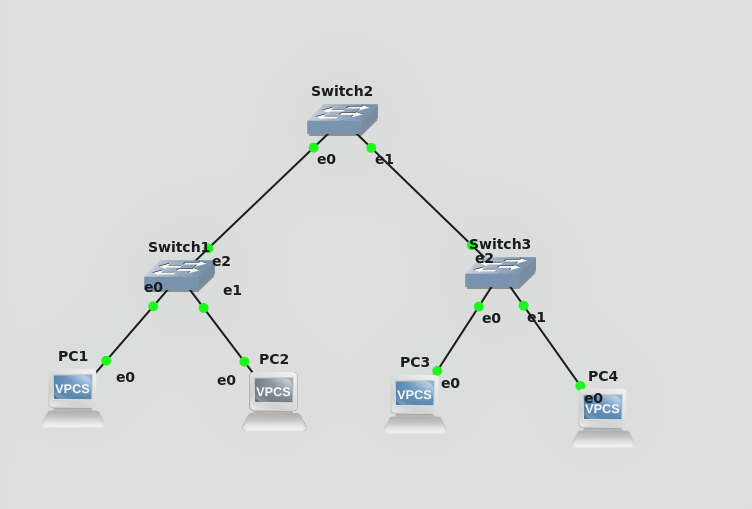
\includegraphics[width=.45\textwidth]{network.png}
        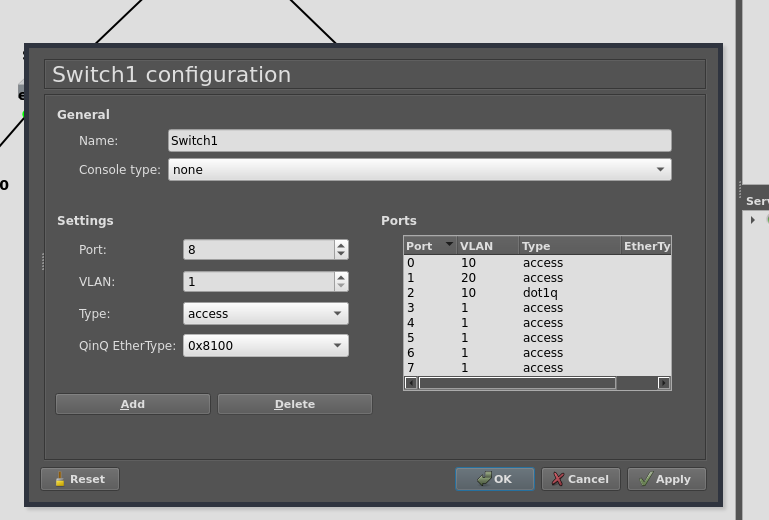
\includegraphics[width=.45\textwidth]{switch1.png}
        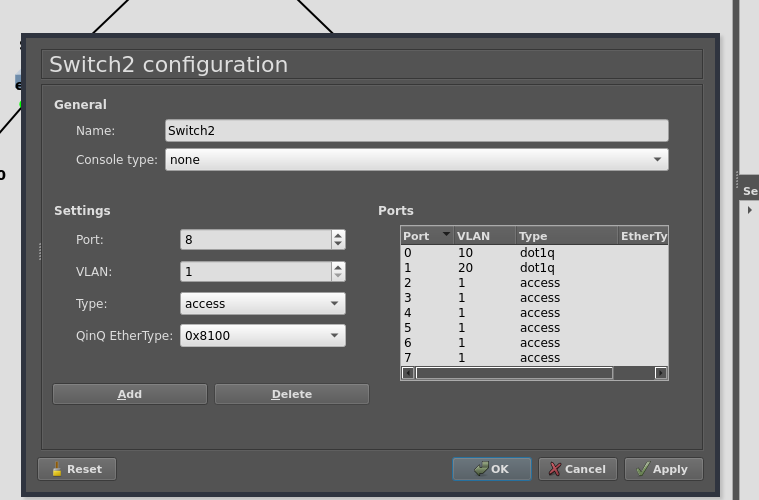
\includegraphics[width=.45\textwidth]{switch2.png}
        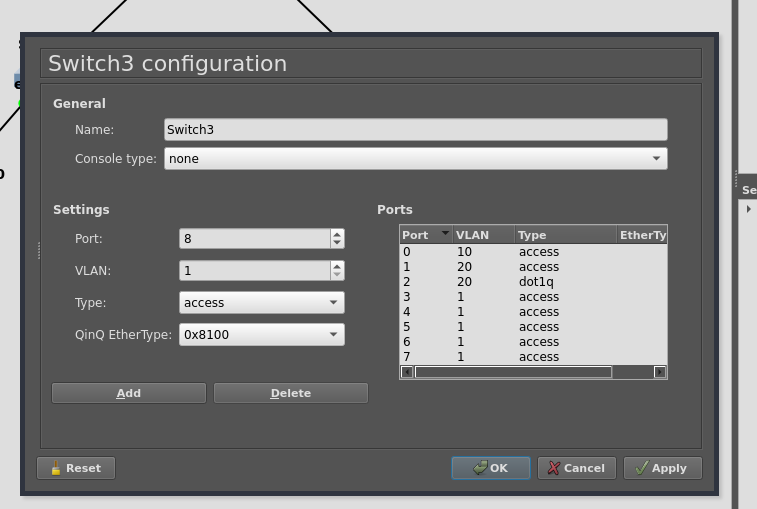
\includegraphics[width=.45\textwidth]{switch3.png}
    \end{center}

    \item Jeweils (PC1 und PC3), und (PC2 und PC4) sind wechselseitig erreichbar weil sie im selben VLAN (10 bzw. 20) sind.
    
    \item Nur zwischen Switch2 und Switch3 wurde VLAN-Information mitgesendet. PC1 weiss nichts von VLAN, sendet also keine mit. Switch1 erhält Pakete von PC1 auf Port 0, der VLAN 10 zugeordnet ist. VLAN 10 ist aber auch sein natives VLAN, also schickt er das Paket ohne Tag weiter an Switch2.
    
    \begin{center}
        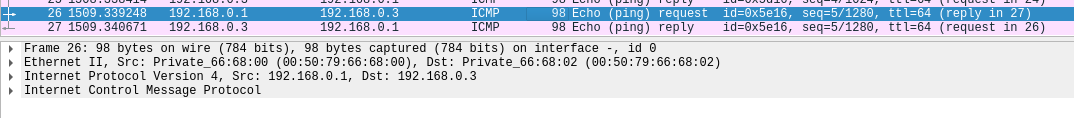
\includegraphics[width=.9\textwidth]{pc1-pc3-noflag.png}
        Paket zwischen PC1 und Switch1    
    \end{center}

    Switch2 erhält das nicht mit Tag versehene Paket auf VLAN 10, sein natives VLAN ist 20 also schickt er es mit Tag VLAN 10 weiter an Switch3.

    \begin{center}
        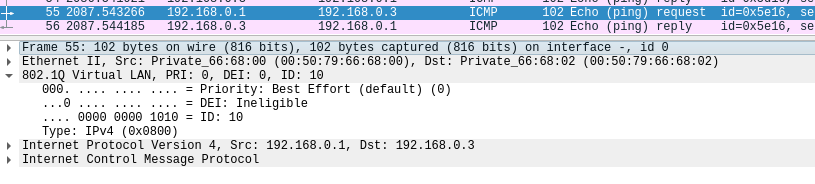
\includegraphics[width=.9\textwidth]{pc1-pc3-flag.png}
        Paket zwischen Switch2 und Switch3, mit ID: 10 wird das VLAN des Pakets vermerkt 
    \end{center}

    Switch3 erhält das Paket und schickt es an PC3, dabei wird das Tag nicht mitgesendet, PC3 muss/soll nichts von VLANs wissen.

    \item Dieses mal wird nur zwischen Switch1 und Switch2 ein VLAN-Tag mitgesendet. Wieder schickt der PC kein VLAN Tag. Switch1 erhält nun auf Port 1 Pakete, also auf VLAN 20. Das ist nicht sein natives VLAN, also schickt er über den Trunk das VLAN Tag mit ID 20 mit.

    \begin{center}
        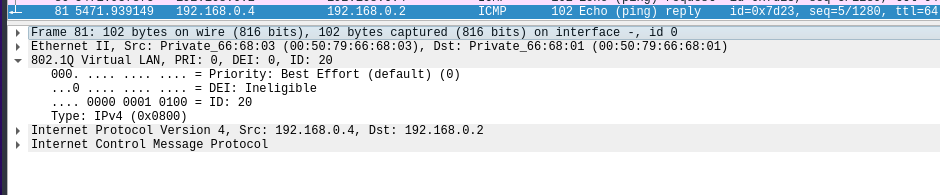
\includegraphics[width=.9\textwidth]{pc2-pc4-flag.png}
        Paket zwischen Switch1 und Switch2, mit ID: 20 wird das VLAN des Pakets vermerkt 
    \end{center}

    Switch2 erhält nun das getaggte Paket und schickt es an Switch3 weiter. Weil aber sein natives VLAN 20 ist, schickt er kein Tag mit. Switch3 schickt das Paket über einen Access Port, also wieder kein Tag.
\end{enumerate}

\paragraph{Aufgabe 2.}
 
\begin{enumerate}[label=(\arabic*)]
    \item Die MAC-Adresse $m$ des Empfängers wird aus dem Frame ausgelesen.
    \item Ist $m$ im internen \emph{address table} so wird das Frame entsprechend der gespeicherten Adresse weitergeleitet (Forwarding). Der address table ist im einfachsten Fall eine key-value Liste, mit Adressen als keys und Ports als values.
    \item Ist $m$ unbekannt so wird das Frame über alle Ports (mit Ausnahme desjenigen, über dem es angekommen ist) ausgesendet (Flooding). Unter der Annahme, dass ein Gerät mit Adresse $m$ im Netzwerk ist, kann so der zum Empfänger führende Port ermittelt und entsprechend in der Liste vermerkt werden (Learning). 
\end{enumerate}

Vor der Weiterleitung inspiziert der Switch üblicherweise das gesamte Frame auf Fehler. 

\end{document}
